\chapter{Lecture 35 - More General Galerkin Finite Element Methods}
\label{ch:lec35n}
\section{Objectives}
The objectives of this lecture are to:
\begin{itemize}
\item Illustrate the application of the FEM for problems with type-2 and type-3 boundary conditions.
\item Discuss issues relevant for analysis of more general partial differential equations with the FEM.
\end{itemize}
\setcounter{lstannotation}{0}

\section{Problem Statement}
In the last lecture we solved a problem that had only type-1 boundary conditions.  In this lecture we will show how to solve problems with type-2 and type-3 boundary conditions.  

For this exercise we will re-solve a problem that we first met in Lecture 30. Consider the nuclear fuel pin depicted in Figure \ref{fig:lec35n-ex1-schematic}.  As described in Lecture 30,  heat is generated by fission in the cylindrical fuel pellet; this heat is conducted through the fuel and cladding and dissipated to coolant flowing along the outside of the fuel pin.  Prompt fission gamma rays also deposit energy in the cladding due to photon interactions with the clad material.  The outer surface of the cladding is cooled by flowing water at $T_{\infty}=473$K with heat transfer coefficient of $h=10^4\ \text{W/m}^2\text{-K}$.  The thermal conductivity of the cladding material is $k=16.75 \ \text{W/m-K}$.  The dimensions of the fuel rod are $R=1.5\times 10^{-2}\text{ m}$, and $w=3.0\times 10^{-3}\text{ m}$.  At steady-state, conservation of energy in the cladding can be expressed by the following boundary value problem:
\begin{marginfigure}
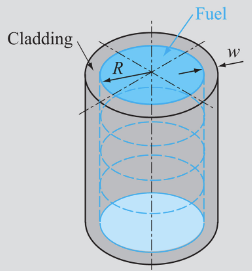
\includegraphics{lec30n-ex1-schematic.png}
\caption{A typical nuclear reactor fuel pin.}
\label{fig:lec35n-ex1-schematic}
\end{marginfigure}
\begin{table}[h!]
\begin{tabular}{l l}
ODE: & $\frac{1}{r}\frac{d}{dr}\left(rk\frac{dT}{dr}\right)=-10^8\frac{e^{-r/R}}{r}, \ \  R < r < R+w $ \\
BCs: & $\frac{dT}{dr}\Bigl|_{r=R}=-\frac{6.32\times 10^5}{k}, \ \ \frac{dT}{dr}\Bigl|_{r=R+w}=-\frac{h}{k}\left(T(r+w)-T_{\infty}\right)$ \\
\end{tabular}
\end{table}

\newthought{Recall that in} Lecture 30, we re-expressed the governing equation so it would be ammenable to solution with \lstinline[style=myMatlab]{bvp5c}.  As a result, the governing equation can be equivalently written as shown in Equation \ref{eq:lec35n-gov-eq}.
\begin{equation}
\frac{d^2T}{dr^2}+\frac{1}{r}\frac{dT}{dr} = -\frac{10^8e^{-r/R}}{rk}
\label{eq:lec35n-gov-eq}
\end{equation}

We start by expressing this equation in the strong form of the weighted residual statement:\marginnote{

\noindent\textbf{Note:} We change our convention and denote the test function with $v$ since the character $w$ is already used to indicate the clad thickness.

}
\begin{equation*}
\int_{R}^{R+w} v \frac{d^2T}{dr^2} \ dr + \int_{R}^{R+w} v \frac{1}{r}\frac{dT}{dr} \ dr + \int_{R}^{R+w} v \frac{10^8e^{-r/R}}{rk} \ dr = 0
\end{equation*}
We convert this to the weak form by carrying out integration by parts on the first term.  The result is:
\begin{multline*}
\underbrace{v(R+w) \frac{dT}{dr}\Bigl|_{r=R+w} - v(R)\frac{dT}{dr}\Bigl|_{r=R}}_{\text{boundary terms}} \\
-\int_{R}^{R+w} \frac{dv}{dr}\frac{dT}{dr} \ dr +  \int_{R}^{R+w} v \frac{1}{r}\frac{dT}{dr} \ dr + \int_{R}^{R+w} v \frac{10^8e^{-r/R}}{rk} \ dr = 0
\end{multline*}

\noindent We can substitute the given boundary conditions into the boundary terms of the weak form:
\marginnote{
\noindent\textbf{Note:} the result of evaluating each boundary term will be a scalar so they ultimately will be placed on the right-hand side (RHS) vector.  The term evaluated at $r=R$ will be added to the first element of the RHS since it is associated with the first equation; the term evaluated at $r=R+w$ will be added to the last RHS element since it is associated with the last degree of freedom (and hence last equation).  

\vspace{0.2cm}

\noindent The terms ``kernel \#1'' and ``kernel \#2'' are so labeled because they involve both the trial function and test function; the resulting submatrices will be added to the system matrix.  The term labeled ``source'' is so named because it does not involve the trial function; the integral will result in a vector that will be incorporated into the RHS.  
}
\begin{multline*}
\underbrace{v(R+w) \left[-\frac{6.32\times 10^5}{k} \right] - v(R)\left[-\frac{h}{k}\left(T(r+w)-T_{\infty}\right) \right]}_{\text{boundary terms}} \\
-\underbrace{\int_{R}^{R+w} \frac{dv}{dr}\frac{dT}{dr} \ dr}_{\text{kernel \#1}} +\underbrace{\int_{R}^{R+w} v \frac{1}{r}\frac{dT}{dr} \ dr}_{\text{kernel \#2}} +\underbrace{\int_{R}^{R+w} v \frac{10^8e^{-r/R}}{rk} \ dr}_{\text{source term}} = 0
\end{multline*}
Now the problem is in a form that can be solved using the FEM.

\section{Matlab Solution}
Almost all of the code used for the second example in Lecture 34 can be re-used.  We start by clearing out the workspace and introducing problem-specific parameters.  Almost all of the remainder of the code is re-used.  The only part that needs to be specialized is for calculation of, what we have dubbed, the kernels and the source term.  



\begin{lstlisting}[style=myMatlab,name=lec35n-ex]
clear
clc
close 'all'

%% Parameters
R = 1.5e-2; % m, radius of fuel
w = 3.0e-3; % m, thickness of cladding
k = 16.75; % W/(m-K), thermal conductivity of clad
Q = 1e8; % W/m^2, Source term from heat dep in cladding.
Q2 = 6.32e5; % W/m^2, Heat flux due to heat produced in fuel.
T_inf = 423; % K, temperature of water flowing on cladding
h = 1e4; % W/(m^2-K), convective heat transfer coefficient

a = R; b = R+w;
\end{lstlisting}

\marginnote{

\vspace{3.5cm}

\noindent\ref{lst:ann35n-1} This portion of the listing is completely re-used.

}
\begin{lstlisting}[style=myMatlab,name=lec35n-ex]
% initialize global arrays
K1 = zeros(nnodes,nnodes);
K2 = zeros(nnodes,nnodes);
S1 = zeros(nnodes,1);

% carry out assembly process
for ele = 1:nelem

    % local arrays to be populated  /*!\annotation{lst:ann35n-1}!*/
    k1 = zeros(nldofs,nldofs);
    k2 = zeros(nldofs,nldofs);
    s1 = zeros(nldofs,1);
    
    % local mapping for GQ
    aL = gcoord(nodes(ele,1));
    bL = gcoord(nodes(ele,end));
    xT = @(t) ((bL - aL)*t + aL + bL)/2;
    Jac = (bL - aL)/2;

    % Get vector of sample points for shape functions
    xgl = gcoord(nodes(ele,:));
    
    % get Lagrange Interpolant of requested order
    H = getLagrangeInterp(xgl);
    Hp = getLagrangeInterpDeriv(xgl);
\end{lstlisting}

In this next section, we carry out the calculations for the elements of the weak form of the minimum weighted residual statement.

\marginnote{

\vspace{1.4cm}

\noindent\ref{lst:ann35n-2} We introduce this variable: a) to improve readability; and b) to avoid re-computing \lstinline[style=myMatlab]{xT(q(qp))} numerous times within the loop.

\vspace{0.1cm}

\noindent\ref{lst:ann35n-3} Compute the contribution to kernel \#1.

\vspace{0.3cm}

\noindent\ref{lst:ann35n-4} Compute the contribution to kernel \#2.

\vspace{0.6cm}

\noindent\ref{lst:ann35n-5} Compute the contribution to the source term.
}
\begin{lstlisting}[style=myMatlab,name=lec35n-ex]
    for qp = 1:nqp
        
        % sum weighted contribution at Gauss Points
        xqp = xT(q(qp)); /*!\annotation{lst:ann35n-2}!*/
        for i = 1:nldofs
            for j = 1:nldofs
                
                k1(i,j) = k1(i,j) + ...    /*!\annotation{lst:ann35n-3}!*/
                    Hp{i}(xqp)*Hp{j}(xqp)*w(qp);
                                
                k2(i,j) = k2(i,j) + ...    /*!\annotation{lst:ann35n-4}!*/
                    (1./xqp)*H{i}(xqp)*Hp{j}(xqp)*w(qp);
            end % j
            c = (1./xqp)*(1/k)*Q*exp(-xqp/R);
            s1(i) = s1(i) + c*H{i}(xqp)*w(qp);  /*!\annotation{lst:ann35n-5}!*/
        end % i
     
    end % qp
    % apply Jacobian to map to physical coordinates
    k1 = k1*Jac;
    k2 = k2*Jac;
    s1 = s1*Jac;

\end{lstlisting}
Now that the subarrays for the kernels and source term are computed for the element, we add them to the global arrays.

\marginnote{

\vspace{3.85cm}

\noindent\ref{lst:ann35n-6} For loops that extend over longer code segments, it is a good practice to leave a comment like this to help clarify which loop is being ended.

\vspace{0.25cm}

\noindent\ref{lst:ann35n-7} The signs used here are from the weak form. Alternatively the signs could be incorporated into the calculation of each kernel element.  For the source term, the negative sign comes from moving it to the RHS.

\vspace{0.25cm}

\noindent\ref{lst:ann35n-8} Be very careful with signs here as well.  Both terms get moved to the RHS and placed in the element of the RHS vector based on the degree of freedom on which they operate.  The part of the type-3 boundary condition that multiplies by the dependent variable, needs to be added to the system matrix.
}
\begin{lstlisting}[style=myMatlab,name=lec35n-ex]
    % add local arrays to global arrays "assembly"
    for i = 1:nldofs
        for j = 1:nldofs
            row = nodes(ele,i); col = nodes(ele,j);
            K1(row,col) = K1(row,col) + k1(i,j);
            K2(row,col) = K2(row,col) + k2(i,j);
        end % j
        dof = nodes(ele,i);
        S1(dof) = S1(dof) + s1(i);
    end % i

end % numel /*!\annotation{lst:ann35n-6}!*/

% apply boundary conditions
A = -K1 + K2;  /*!\annotation{lst:ann35n-7}!*/
RHS = -S1;

% provide contributions from boundary conditions
c1 = Q2/k;
RHS(1)=RHS(1)-c1;

c2 = h/k;       /*!\annotation{lst:ann35n-8}!*/
RHS(nnodes)=RHS(nnodes)-c2*(T_inf);
A(nnodes,nnodes) = A(nnodes,nnodes)-c2;

% solve the system of equations
u = A\RHS;
\end{lstlisting}

The solution computed using the finite element method, as expected, matches the solution we obtained with \lstinline[style=myMatlab]{bvp5c} back in Lecture 30 and is shown in Figure \ref{fig:lec35n-ex-sol}.
\begin{marginfigure}
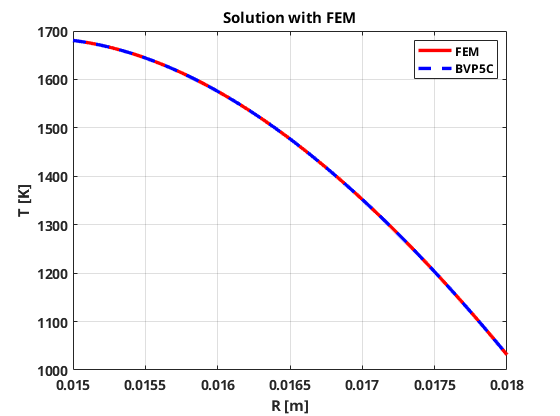
\includegraphics{lec35n-ex-sol.png}
\caption{Comparison of solutions for the example problem.}
\label{fig:lec35n-ex-sol}
\end{marginfigure}

\section{Generalizing Finite Element Methods}
In the classroom version of this course, the exposition presented here is followed by a sequence of workshops where students learn to use, with a basic level of proficiency, a generalized FEM package like COMSOL.  In this section we will broaden our area of focus and discuss the aspects of FEM technology that are required to address more general classes of problems.

\subsection{The Weak Form for Partial Differential Equations}
The problems we have solved so far have been greatly simplified by the fact that they are all posed in one spatial dimension.  The geometry is easy to describe, the boundaries are easy to identify and the calculus involved in converting the strong form into the weak form is more simple. 

\newthought{To illustrate the} process of converting from the strong form to the weak form in two dimensions, let us consider a boundary value problem based on the Laplace equation that we solved in Lecture 26 of the analytical methods part of the text:
\begin{table}[h]
\begin{tabular}{l l}
$\substack{\text{Governing} \\\text{Equation}}: $& $\frac{\partial^2 u}{\partial x^2} + \frac{\partial^2 u}{\partial y^2} = 0, \ \ 0<x<a, \ \ 0<y<b $\\
& \\
$\substack{\text{Boundary} \\ \text{Conditions}}: $ & $\substack{u(x,0)=0  \ \ \ \ \ \ u_x(0,y) = 0 \\ \\ u(x,b) = f(x) \ \ u_x(a,y) = 0}$ 
\end{tabular}
\end{table} 
where a schematic of the domain and boundary conditions is shown in Figure \ref{fig:lec35n-ex2-schematic}.
\begin{marginfigure}
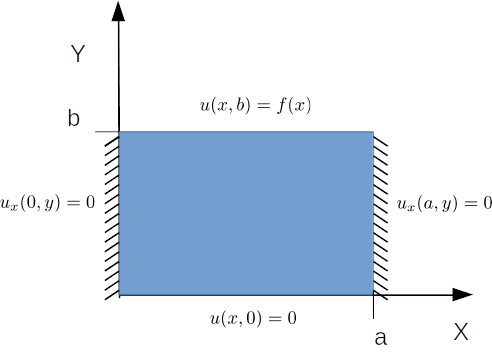
\includegraphics{lec26_fig1.png}
\caption{Schematic of example Laplace's equation problem.}
\label{fig:lec35n-ex2-schematic}
\end{marginfigure}  


